% !TEX program = xelatex
\documentclass[11pt,a4paper]{ctexart}
\usepackage[margin=1in]{geometry}
\usepackage{graphicx}
\usepackage{booktabs}
\usepackage{amsmath,amssymb}
\usepackage{algorithm}
\usepackage{algpseudocode}
\usepackage{hyperref}
\usepackage{natbib}
\usepackage{xcolor}
\usepackage{caption}
\usepackage{subcaption}

\title{面向终身多智体取送货的可解释车队并发控制：基于会商的混合规划}
\author{匿名作者\\投稿准备稿（草稿）}
\date{}

\begin{document}
\maketitle

\begin{abstract}
终身多智体取送货（Lifelong MAPD）要求在碰撞约束下持续分配并执行取货—送货任务。基于搜索的窗口求解器（如 RHCR 结合 ECBS）完成率高但墙钟昂贵；反应式方法（如 PIBT）速度快，却在容量为 1 的走廊中脆弱。本文提出 \emph{Meeting-RH} 混合栈：将慢变量——阶段位姿、优先级与短视窗提交——与快速冲突修复分离，并引入两个带几何门控的小型模仿学习模块。\textbf{StageNet} 在 FINAL~/~APPROACH~/~CLEAR 阶段间选择并输出优先级；\textbf{FACN} 预测离散并发残差 $\Delta$，将喉带容量调整为 $K=\mathrm{clip}(K_{\mathrm{TBC}}+\Delta)$，且不改动路径代价。几何门控协议对应可复现失败模式，无需地图 ID 硬编码。在含每图约 100 条终身任务的 20 图压力套件上，本方法在 VALID 与全量完成上与 ECBS/Hier 持平，平均仿真时间约为分层 ECBS 的 42\%，墙钟时间降低 1--2 个数量级。
\end{abstract}

\noindent\textbf{关键词：}终身 MAPD；多智体路径规划；滚动视窗；模仿学习；车队规模；可解释协同

\section{引言}
多智体路径规划（MAPF）要求共享图上无碰撞路径~\citep{sharon2015cbs,stern2019mapf}。仓储场景通常需要\emph{终身}变体~\citep{ma2017mapd2,li2021rhcr}。基于搜索的方法有效性强但墙钟开销大~\citep{barer2014ecbs,li2021rhcr}；反应式方法如 PIBT 可扩展却在窄喉退化~\citep{okumura2022pibt}。RHCR 仅在窗口内消解冲突~\citep{li2021rhcr}，但未显式学习异构几何下应允许多少智体保持忙碌~\citep{chen2024scaling}。

本文针对\textbf{运营并发度}与\textbf{阶段位姿}：慢、可解释、适合小型监督模型；快速碰撞修复保持算法化。

\paragraph{贡献。}
(1)~\textbf{Meeting-RH 双时间尺度}：$H{=}12$ 会商协商阶段、优先级与窗口时空提交；会商间契约跟进。
(2)~\textbf{FACN}：预测 $\Delta$；$K=\mathrm{clip}(K_{\mathrm{TBC}}+\Delta)$ 门控认领（不选具体车）。
(3)~\textbf{StageNet + ASA}：阶段打分与优先级；ASA 依 $(n,\textit{near})$ 切换网络/教师。
(4)~\textbf{几何门控协议套件}：竞争目的地、垫区出口、FG-CEBI、粘性卸货后出口、进度脉冲、焦点利他等。
(5)~\textbf{实证}：SH01--20 上 VALID$\land$full100 对标 ECBS/Hier，sim/wall 显著更优。

Meeting-RH 相对 CBS \textbf{不完备}；收益为 VALID$\land$全量完成体制内的实用帕累托改进。

\section{相关工作}
\textbf{最优/有界次优 MAPF。} CBS~\citep{sharon2015cbs}、ECBS~\citep{barer2014ecbs,pearl1982focal}。
\textbf{优先/窗口规划。} WHCA*~\citep{silver2005whca}、优先规划~\citep{cap2015prioritized}、RHCR~\citep{li2021rhcr}、经验预热~\citep{madar2022exrhcr}。
\textbf{反应式终身求解器。} PIBT~\citep{okumura2022pibt}；学习增强~\citep{skrynnik2024follow,damani2021primal}。
\textbf{MAPD。}~\citep{ma2017mapd2,liu2019lifelong}。

\section{问题形式化}
四连通网格 $G=(V,E)$；车队 $A=\{a_i\}_{i=1}^{n}$。禁止顶点冲突与边交换冲突；取货站 FIFO。\textbf{VALID} 要求运动学、容量与冲突约束均满足。指标：$\textit{done}$、$\textit{full100}$、$\textit{sim}$、$\textit{wall}$。压力图 SH01--20，每图约 100 任务。

\section{方法：Meeting-RH}
\subsection{双时间尺度}
\begin{algorithm}[t]
\caption{Meeting-RH 拍循环（概念）}
\label{alg:meet}
\begin{algorithmic}[1]
\State 初始化契约；$t_{\mathrm{last}}\leftarrow -H$
\For{$t=0,1,2,\ldots$}
  \If{会商触发（$t{-}t_{\mathrm{last}}\ge H$ 或停滞/无进展）}
    \State $K\leftarrow\mathrm{clip}(K_{\mathrm{TBC}}+\mathrm{FACN}(g,x))$（含 AFA）
    \State 阶段、优先级 $\leftarrow$ ASA(StageNet, 教师)
    \State 应用目的地门、垫区出口、区域准入
    \State 优先序时空 BFS，视窗 $W\in\{16,28\}$
    \State 修复窗口；签发 StageContract（TTL${=}16$）
    \State $t_{\mathrm{last}}\leftarrow t$
  \EndIf
  \State 跟进提交；空隙让行；可选 PGFA；拍协议
\EndFor
\end{algorithmic}
\end{algorithm}

\textbf{慢（会商）：}路径缓存；ASA；区域软准入；竞争目的地/垫区出口；\textbf{窗口时空 BFS}；修复；双字典序合法化（$10\le n\le 14$）；契约 TTL${=}16$。
\textbf{快：}跟进提交头；空隙让行；PGFA 帮单一焦点。

相对 RHCR~\citep{li2021rhcr}：协商紧凑慢变量，而非每周期调用完整联合窗口 MAPF。

\subsection{几何门与 FACN}
Multi-Band TBC 给出 $K_{\mathrm{TBC}}$。FACN：$[g;x]\in\mathbb{R}^{22}\to\Delta$。AFA 防抖动。认领服从 $K$；BFS 边代价不变。

\subsection{StageNet}
候选：FINAL、APPROACH@$1/3$、$2/3$、CLEAR。特征 $x_a\in\mathbb{R}^{8}$。MLP $8{\to}64{\to}64$。ASA 在噪声体制（常 $n\le 9$）切回教师。

\subsection{协议套件}
竞争目的地门；垫区出口与 FG-CEBI；E4；进度脉冲；PGFA；DLO；区域准入。走廊向子集称 \textbf{PGCP}。

\begin{figure}[t]
\centering
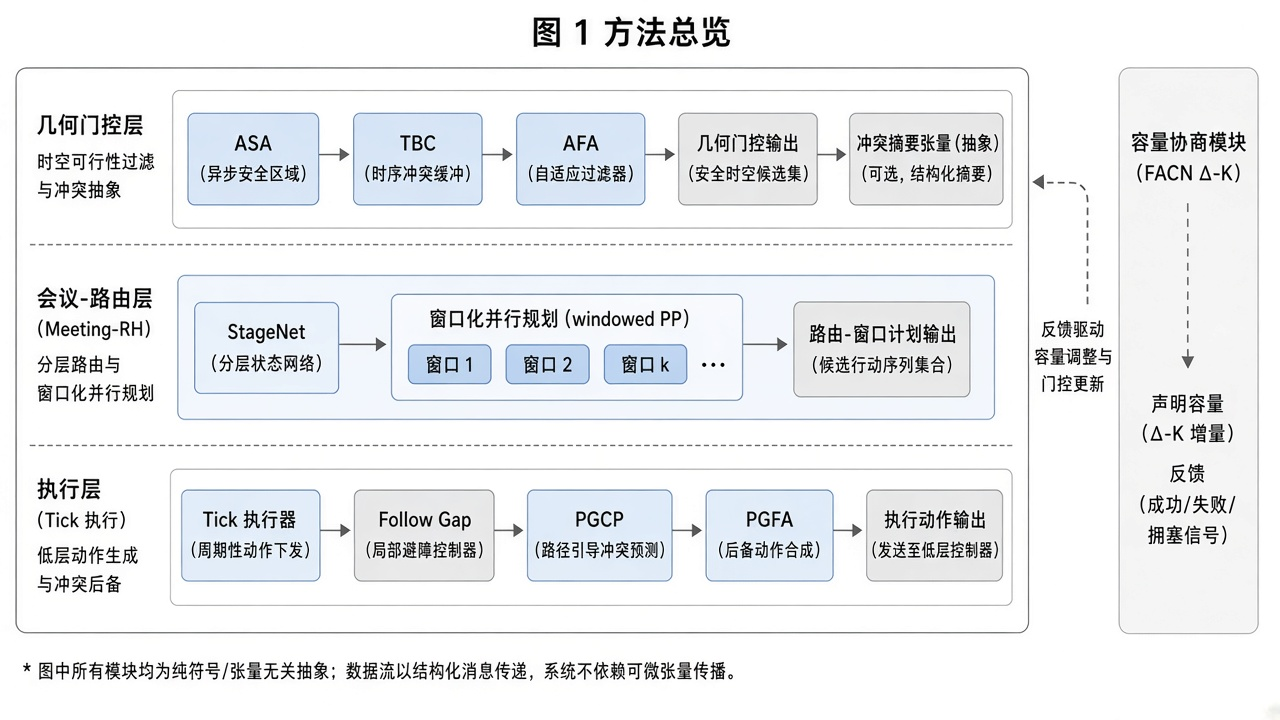
\includegraphics[width=0.95\linewidth]{../figures/fig1_overview_zh.jpg}
\caption{Meeting-RH 栈：几何门、会商、拍执行与 FACN 对 $K$ 的反馈。}
\label{fig:overview}
\end{figure}

\begin{figure}[t]
\centering
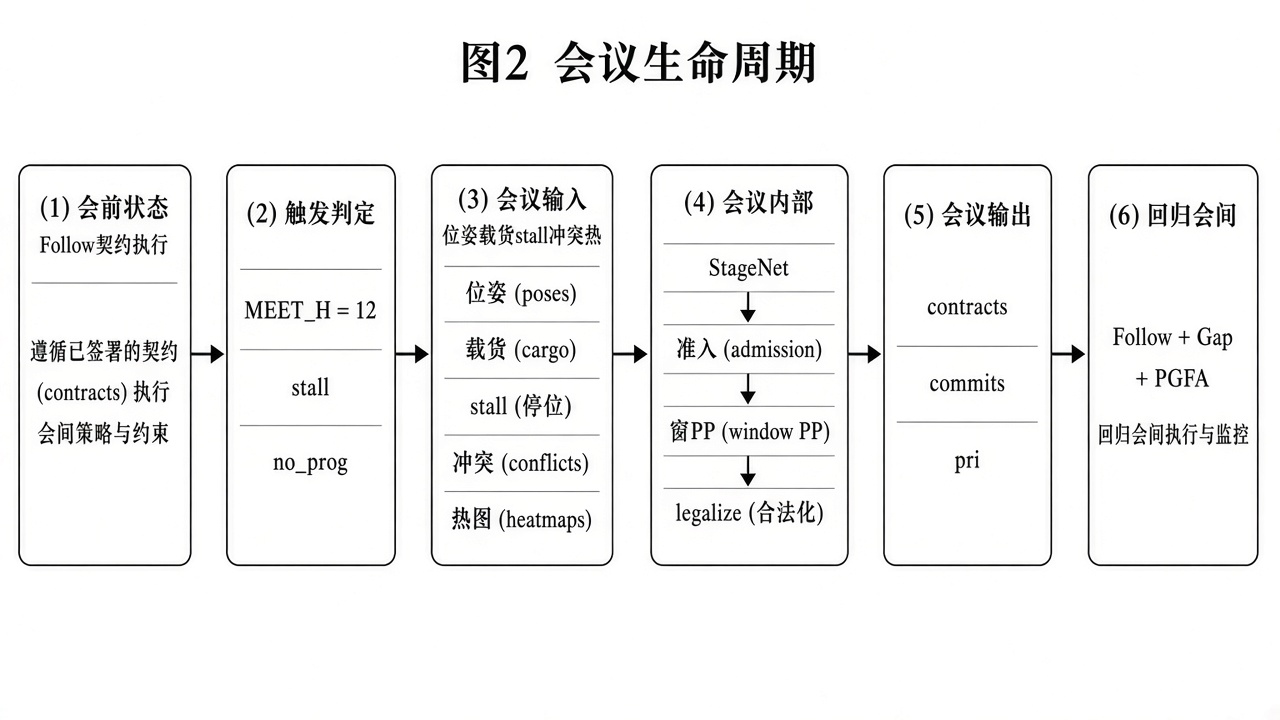
\includegraphics[width=0.95\linewidth]{../figures/fig2_meeting_zh.jpg}
\caption{会商生命周期：预跟进 $\to$ 触发 $\to$ 输入 $\to$ 内部步骤 $\to$ 契约。}
\label{fig:meeting}
\end{figure}

\section{实验}
\subsection{设置}
基线：PIBT、M0、PP、窗口 ECBS、Hier。本文：Meeting-RH + 协议 + StageNet（ASA）+ FACN（AFA）。\texttt{PYTHONHASHSEED=0}；CPU；每图子进程。

\subsection{主结果}
\begin{table}[t]
\centering
\caption{SH01--20（官方 100）汇总。VALID$\land$full100 中 sim/wall 越低越好。$^\dagger$未全完成图上的 sim 不可作“更快”解读。}
\label{tab:main}
\begin{tabular}{lccccc}
\toprule
方法 & full100 & VALID & avg\_done & avg\_sim & avg\_wall \\
\midrule
PIBT & 8/20 & 20/20 & 63.9 & 62811 & 40.5s \\
M0 & 4/20 & 20/20 & 44.6 & 942$^\dagger$ & 1478s \\
PP & 1/20 & 7/20 & 32.4 & 848$^\dagger$ & 1716s \\
ECBS & 20/20 & 20/20 & 100 & 7364 & 543s \\
Hier & 20/20 & 20/20 & 100 & 4018 & 1032s \\
\textbf{本文} & \textbf{20/20} & \textbf{20/20} & \textbf{100} & \textbf{1708} & \textbf{$\sim$28s} \\
\bottomrule
\end{tabular}
\end{table}

在 20/20 全完成方法中，本文 avg\_sim 约为 Hier 的 42\%、ECBS 的 23\%，墙钟约 28s。仅协议相对旧 FULL：约 $-9.0\%$ avg\_sim、0 图变差。FACN v2 相对 noFACN（SH01--40）：约 $-5.82\%$ avg\_sim。

\subsection{消融}
关 StageNet：难图崩溃（SH10 done 60；SH17 done 32）。关 PGCP：SH10/11/12/17 完成率下降。关 PGFA：SH17 done 20。关 FACN：开阔大车队受损（SH20 $660\!\to\!813$）。

\begin{figure}[t]
\centering
\begin{subfigure}{0.48\linewidth}
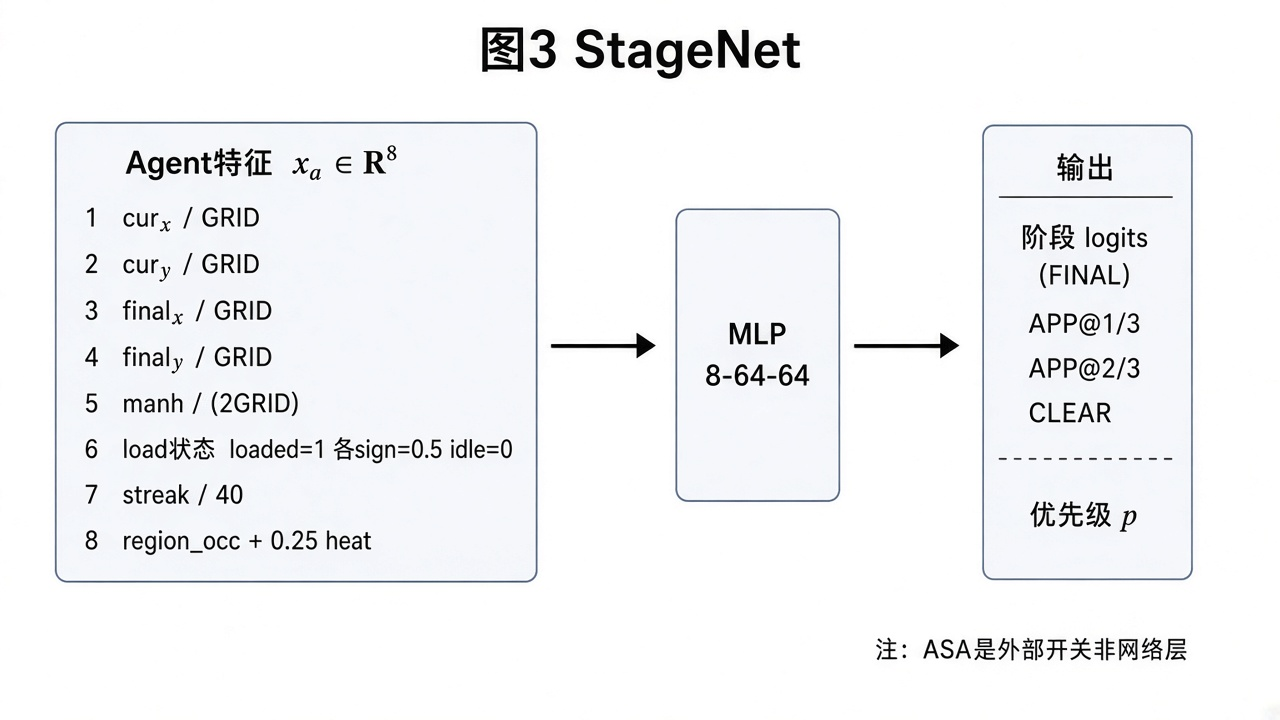
\includegraphics[width=\linewidth]{../figures/fig3_stagenet_zh.jpg}
\caption{StageNet 输入输出}
\end{subfigure}
\hfill
\begin{subfigure}{0.48\linewidth}
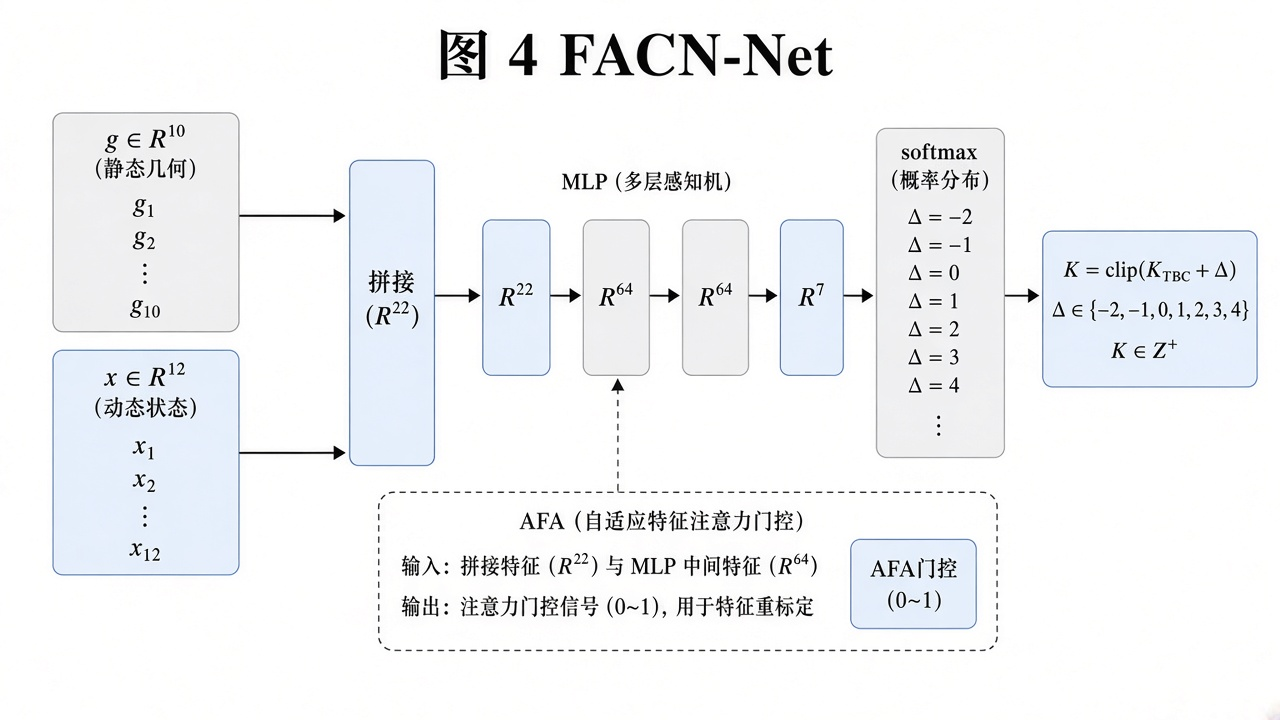
\includegraphics[width=\linewidth]{../figures/fig4_facn_zh.jpg}
\caption{FACN 输入输出}
\end{subfigure}
\caption{Meeting-RH 使用的小型模仿模块。}
\label{fig:nets}
\end{figure}

\subsection{为何窗口 BFS 优于串行 M0 A*}
M0 反复跑\textbf{全视界时空 A*}；Meeting-RH 多数时间契约跟进，会商仅在 $W$ 内做\textbf{优先序时空 BFS}。

\section{局限}
相对 CBS 不完备；FACN 留出泛化有限；协议可相互作用；压力图$\neq$工业数字孪生。

\section{结论}
Meeting-RH 将几何门控协议与 StageNet、FACN 耦合，用于可解释终身 MAPD。实证上对标强搜索基线的有效性与完成率，同时改善仿真与墙钟。未来工作包括更强留出并发学习与 anytime 窗口搜索集成~\citep{li2021mapflns}。

\bibliographystyle{plainnat}
\bibliography{../refs}

\end{document}
